\section*{Problem 6}

Find the Fourier transform of the following signals. Sketch $|X(\omega)|$ in each case.

\begin{enumerate}
%%%%%%%%%%%%%%%%%%%%%%%%%%%%%% a %%%%%%%%%%%%%%%%%%%%%%%%%%%
\item :
\begin{figure}[H]
\caption*{}
\centering
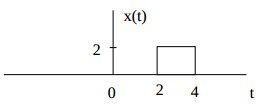
\includegraphics[width=0.4\textwidth]{figs/c2p6a.png}
\label{fig:c2p6a}
\end{figure} 
\subsection*{Solution}

Lets call $x_{p1}(t)$ and $X_{p1}(\omega)$ the function in time domain of the first point 
and its Fourier Transform respecively. 
We can express our function in terms of such function as:

\begin{equation*}
x(t) = x_{p1}(t-2)
\end{equation*} 

As we can see from (\ref{eq:c22b}) the displacement in time is reflected in the
frecuency domain as a multiplication by an exponential. 

\begin{equation*}
\begin{aligned}
X(\omega) &= X_{p1}(\omega) e^{- 2 j \omega} \\
&= 4 Sa(\omega) e^{-3 j \omega}
\end{aligned}
\end{equation*} 

The plot of the magintude of $X(\omega)$ is:
\zcodemat{sources/c2p6a.m}{Plot of Magnitude}

\begin{figure}[H]
\caption{Magnitude $|X(\omega)|$}
\centering
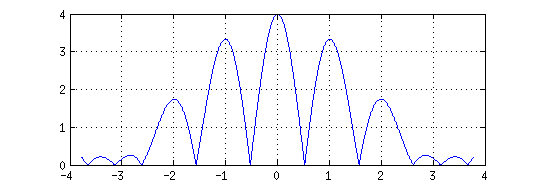
\includegraphics[width=0.8\textwidth]{figs/c2p6a1.png}
\label{fig:c2p6a1}
\end{figure} 

%%%%%%%%%%%%%%%%%%%%%%%%%%%%%% b %%%%%%%%%%%%%%%%%%%%%%%%%%%
\item $x(t) = 2 e^{-2 t} u(t)$
\subsection*{Solution}
Directly from (\ref{eq:c2p5}) we have:
\begin{equation*}
X(\omega) = \frac{2}{2 + j\omega}
\end{equation*} 

The plot of the magintude of $X(\omega)$ is:
\zcodemat{sources/c2p6b.m}{Plot of Magnitude}

\begin{figure}[H]
\caption{Magnitude $|X(\omega)|$}
\centering
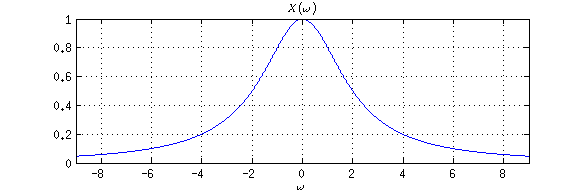
\includegraphics[width=0.8\textwidth]{figs/c2p6b.png}
\label{fig:c2p6b}
\end{figure} 

%%%%%%%%%%%%%%%%%%%%%%%%%%%%%% c %%%%%%%%%%%%%%%%%%%%%%%%%%%
\item $x(t) = 5 e^{-5 t} u(t)$
\subsection*{Solution}
Directly from (\ref{eq:c2p5}) we have:
\begin{equation*}
X(\omega) = \frac{5}{5 + j\omega}
\end{equation*} 

The plot of the magintude of $X(\omega)$ is:
\zcodemat{sources/c2p6c.m}{Plot of Magnitude}

\begin{figure}[H]
\caption{Magnitude $|X(\omega)|$}
\centering
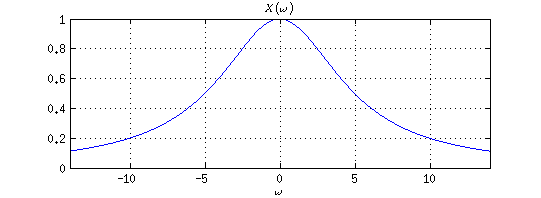
\includegraphics[width=0.8\textwidth]{figs/c2p6c.png}
\label{fig:c2p6c}
\end{figure} 

%%%%%%%%%%%%%%%%%%%%%%%%%%%%%% d %%%%%%%%%%%%%%%%%%%%%%%%%%%
\item $x(t) = e^{-2 t} \cos(4 t) u(t)$
\subsection*{Solution}

\begin{equation*}
x(t) = \frac{1}{2} \left[
	e^{-2t}e^{4j t} u(t) + e^{-2t}e^{-4j t}u(t) \right]
\end{equation*} 

Directly from (\ref{eq:c2p5}) we have:
\begin{equation*}
\begin{aligned}
X(\omega) &= \frac{1}{2} \left[
	\frac{1}{(2 - 4j) +j \omega} + 
	\frac{1}{(2 + 4j) +j \omega} \right] \\
          &= \frac{1}{2} \left[
	\frac{1}{2 + (\omega - 4)j} + 
	\frac{1}{2 + (\omega + 4)j} \right] \\
\end{aligned}
\end{equation*} 

The plot of the magintude of $X(\omega)$ is:
\zcodemat{sources/c2p6d.m}{Plot of Magnitude}

\begin{figure}[H]
\caption{Magnitude $|X(\omega)|$}
\centering
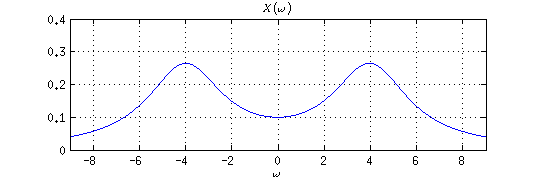
\includegraphics[width=0.8\textwidth]{figs/c2p6d.png}
\label{fig:c2p6d}
\end{figure} 

\end{enumerate} 
